%%%%%%%%%%%%%%%%%%%%%%%%%%%%%%%%%%%%%%%%%%%%%%%%%%%%%%%%%%%%%%%%%%%
%                                                                 %
%                            CHAPTER TWO                          %
%                                                                 %
%%%%%%%%%%%%%%%%%%%%%%%%%%%%%%%%%%%%%%%%%%%%%%%%%%%%%%%%%%%%%%%%%%%

\chapter{PREVIOUS WORK}
%\resetfootnote %this command starts footnote numbering with 1 again.

A number of instances in the literature mentioned previously uses the term versioning and provenance interchangeably.
The version model introduced by Barkstrom in Figure \ref{NASALevels} to organize NASA's satellite data collection actually refers to a simplified workflow describes the provenance used to produce each level of data \cite{Barkstrom2003}.
The diagram does not compare objects from the same level since changes to contributing components are only used as an indicator for version change.
In actuality, objects have much more complicated development structures than the one dimensional lifespan indicated by the transition from Level 0 data to Level 3.
The PROV Ontology model in Figure \ref{PROVO} outlines more explicit inter-relations between data objects, and it provides a new dimension with which to consider the interactions of data objects.
More specifically, it outlines the explicit process of an agent performing an activity using an entity to produce a new entity.
In the context of the level system, an agent (either a program or individual) performs a "Produce Instantaneous Fields" activity using "L1 Data" to produce "L2 Data."
However, higher level data sets rarely use only one instance of lower level data.
Calibration values may result from daily readings collected from another data set, but the generality of the ontology allows these relationships to be explicitly expressed.
A more realistic provenance graph looks like the one in Figure \ref{ProvGraph} of an ozone indicator in which a Level 3 object results from the interrelation of multiple lower level products.
An interesting observation of note is that Tilmes remarks in 2011 \cite{TILMES2011548}, 
\begin{quotation}
	Consider the relatively common case of the calibration table, which is an input to the L1B process, changing. Even though the version of the L2 or L3 software hasn’t changed, the data files in the whole process have been affected by the change in the calibration.
\end{quotation}
which Barkstrom already observes in 2003 \cite{Barkstrom2003}
\begin{quotation}
	If scientific data production were easy, instruments would
	have stable calibrations and validation activities would discover no need for
	corrections that vary with time. Unfortunately, validation invariably shows that
	instrument calibrations drift and that algorithms need a better physical basis. Within a Data Set, we can think of a Data Set Version as a collection of files in
	a Data Set that have a homogeneous Data Production Strategy. Within a Data
	Set Version, we expect the code producing the files to be stable. We also expect
	that the algorithm input coefficients will be stable as well. The intent of data
	production is to produce data whose uncertainties are statistically similar under
	similar conditions of observation.
\end{quotation}
indicating a basic view that despite eight years in difference, the continuation of software focused versioning resulting in difficulties of data oriented collections.

\begin{figure}
	\centering
	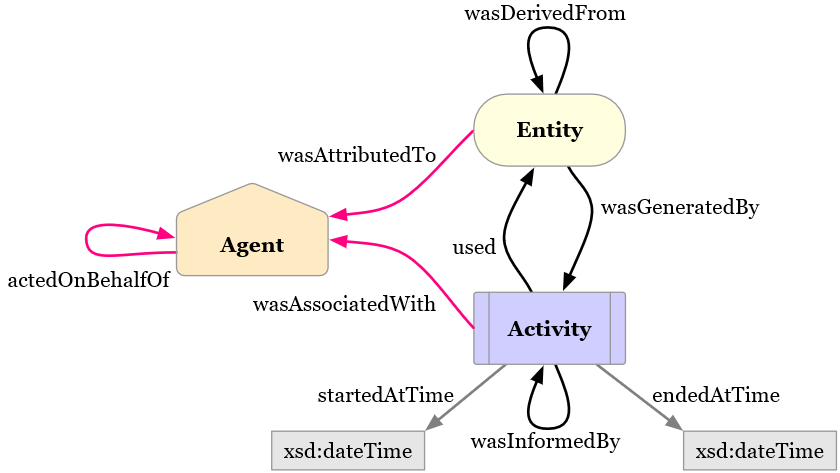
\includegraphics[scale=0.5]{figures/ProvO.png}
	\caption{Diagram of the PROV Ontology.  Figure 1 from \cite{Belhajjame2013b}}
	\label{PROVO}
\end{figure}

\begin{figure}
	\centering
	\begin{adjustbox}{addcode={\begin{minipage}{\width}}{
					\caption{Provenance graph of a Level 3 data product, showing the inter-relations between different data products in generating the final product.  Figure 2 from \cite{TILMES2011548}}\end{minipage}},rotate=90,center}
		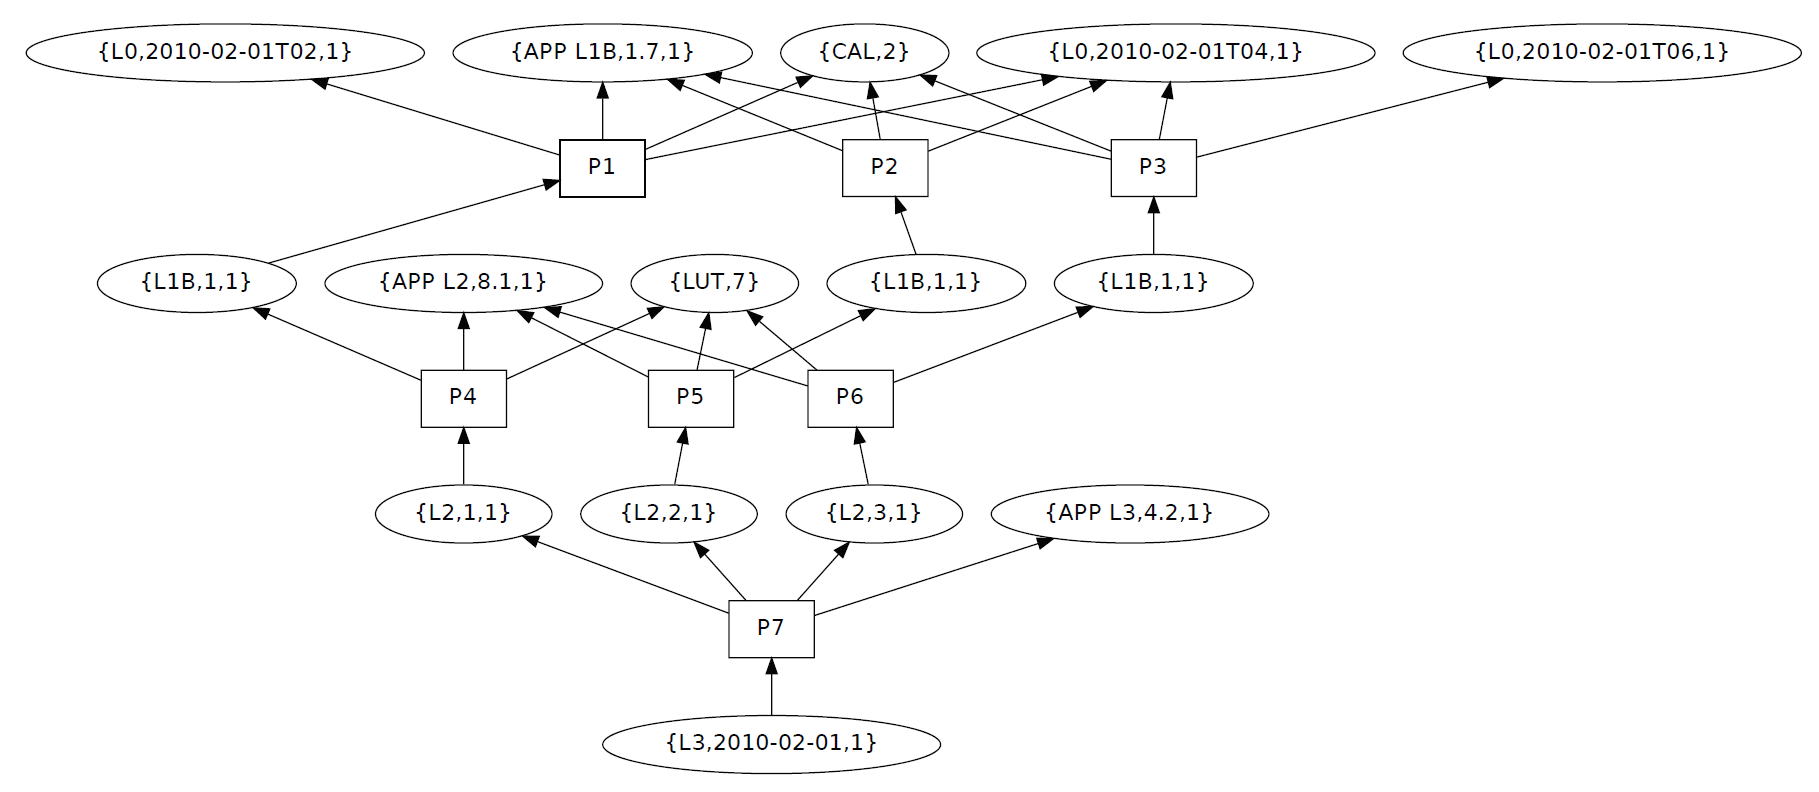
\includegraphics[scale=0.5]{figures/OzoneProvGraph.png}
	\end{adjustbox}
	\label{ProvGraph}
\end{figure}

If the level system provides a length and provenance indicates a breadth of a workflow, a version system can be considered to provide a height to a total workflow.
Referring back to the HCLS data model terminology in Figure \ref{HCLSModel}, as objects within a workflow, as in Figure \ref{ProvGraph}, change versions, the structure of the workflow as well as the Summary Description of the final object, in this case the L3 Ozone product, remains the same.
Instead, the new versions add layers like building blocks over the foundations of the original workflow structure.
Version control systems then provide the mortar linking the blocks together to give the lineage capture procedure a solid structure.
The PAV Ontology provides a means to track versioning information through linked data by introducing \textit{pav:version} to cite versions and \textit{pav:previousVersion} to link them together in order \cite{Ciccarese2013}.
Of note is the retrospective nature \cite{DCMI2012}

\begin{figure}[b]
	\centering
	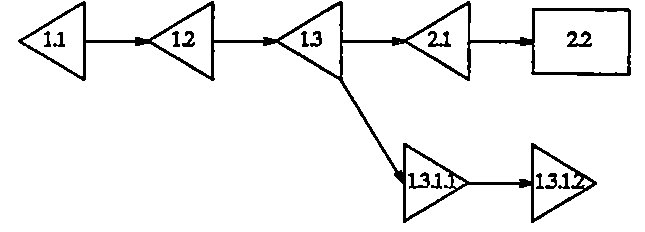
\includegraphics[scale=0.75]{figures/RCSCommitTree.png}
	\caption{Commit history of an object in RCS with changes in the main line stored as back deltas and side branches stored as forward deltas.  Figure 5 in \cite{tichy1985rcs}}
	\label{RCSTree}
\end{figure}


When objects are added to a data set, it does not immediately seem necessary to link the to the older version since the new attribute does not act on the old object.
However, it becomes necessary in order to maintain the history of the flow of changes to the particular work, resulting in the current version as reinforced by PAV
PAV tracks explanations for changes with natural language text comments
PAV directs its trace backwards, whereas this model seeks to communicate forward compatibility

\section{Spreadsheets}

In this project, spreadsheets were chosen for study as they resemble text-like data objects while still maintaining a level of complexities.
Though not as well encapsulated as other data format types such as the Hierarchical Data Format (HDF) or Network Common Data Form (NetCDF), spreadsheets provide many helpful tools that scientist favor for quick data storage and distribution over comma separated values (CSV).
There also exists other document-like formats that are not discussed in this paper such as eXtensible Markup Language (XML).
The initial work was done with the "Noble gas isotope abundances in terrestrial fluids" workbook (Noble Gas) \cite{Polyak2015}.
The "Paragenetic Mode for Copper Minerals" workbook (Copper Data) was used to give better insight into data changes due to collaboration with the data set's author \cite{Morrison2016}.

The Noble Gas data set was initially published on June 11, 2013 and then released a second version on March 8, 2015.
Many significant changes were made to the data set between the two versions, which makes this data set particularly challenging to version.
The physical structure of the data set changed from eight separate Excel spreadsheets to a single spreadsheet.
The second version also trimmed 195 columns to 54 columns in the second release.
In addition, many new locations were surveyed and added to the second release.
Documentation accompanied the data set explaining different components of the spreadsheet and its usage, but it included no versioning information.
This lack of versioning or transitioning information indicates a focus on data usage rather than data maturation, which is not a particularly bad approach.
It makes logical sense to simply download the latest data set when it becomes available and not worry about the format of the invalidated data set.
This approach convenient for new users of the data as the cost to consumer the new version of the data is the same cost they would have spent to acquire the data in the first place.
However, users of the old data are disproportionately effected by the change in versions since old code and workflows may need to be updated to accommodate the changes in addition to the cost of consuming the architecture of the old data set.
In this case, users would need to read the documentation to understand whether 182 from the June data set is still available in the March data and, if it is, in which column it resides in the March spreadsheet.
This brings to light the additional concern for the Noble Gas data that the documentation is not easily machine consumable, meaning that all mapping activities will need to be performed manually.
Not only is this approach time consuming, but it also does not scale well into larger data sets.

The Copper data set was acquired during the process of a workshop to generate new methods of visualizing mineralogy data, initially on June 8, 2016.
The process entailed trying various orders and organization for the data and results in various new versions of the data that depend on varying filtering requirements, acquired on August 21, 2016.
Unlike the Noble Gas data set, the Copper Data had no accompanying documentation, since the primary consumers of the data at the workshop were also mineralogy experts.
However, this data set had more stable characteristics including physical and logical structure.
Only two columns were removed from the transition to the second version, but sixteen new columns were added to the data collection.
It also demonstrates a change in orientation with respect to data usage since the previous data set was designed to be distributed for general usage and discovery.
In this case, the structure and organization of the data within the set was driven for a specific purpose in the development of more expressive visualizations.
As a result, versioning information is driven by developmental needs instead of the other way around with versioning information bridging the gap between software migrations.

The data files from both data sets can easily be tracked using standard version management services such as GIT or SVN.
Likewise, there exist comparison tools like Spreadsheet Compare from Microsoft Corporation that can generate diff-like outputs for each of the data sets.
In conjunction with commit logs, the comparison outputs provide a basic versioning methodology that describes the data set's evolution.
However, these applications rely on human attention and interaction to operate, and with larger data sets, proper documentation becomes difficult to maintain.
With the Copper Data, the demand for new versions of the spreadsheets exceeded the time necessary to document version history as a result of rapid product evolution during the workshop.
In consequence, the process to manually commit and annotate changed data impairs the natural progression of scientific development.

\section{Database Systems}

Databases remain the most relied upon technology for storing and searching large quantities of data rapidly.
While the dynamic combination of tables means that data bases remain flexible enough to represent complex objects, it also means that they represent a much more complicated case for attribution.
Since tables may be combined in different ways to answer complex queries, indexes do not remain constant across requests to the database.
The approaches to database versioning typically focus on ensuring the reproducibility of queries to the database.
This can often be difficult as with spreadsheets since changes to the content or structure can result in different solutions from the database for the same query even using time stamps.
For example, consider the query to select all columns of row A from a database on March 1st, then the database undergoes a schema change to add a new column to the table on April 1st.
A subsequent request for all columns of row A would include the new column which does not represent the response on March 1st.
In addition, even if the data is timestamped, the time signature is associated with the row and not the schema, meaning that the query may still return row A with the new column with a NULL value, depending on the distribution.
The query, not the data, would need to be modified to exclude the new column.

This presents as a challenge because unlike data files and spreadsheets, databases are generally not instanced.
Databases often store massive quantities of data and replication of that data to archive snapshots or distribution frequently proves too costly to be feasible.
Instead, interaction with the database occurs from a centralized source through transactions.
Various methods have been studied to manage changes within these systems focusing primarily on schema versioning, emphasizing data's structural component \cite{roddick1996model}.
This provides a method to enact a transactional rollback on the database to execute queries in an environment reminiscent of the original execution.
The framework of the resulting database environment can become quite complicated as a result of the complexity of the tables representing intricate data objects \cite{Klahold:1986:GMV:645913.671314}.
This results from the need to manage the time instances of realization, storage, and validity.
The datum becomes realized at collection, then stored upon entry into the database, and finally valid until the present or new data replaces it.
More recently, new methods have been developed to adjust to the enormous quantities of data populating modern databases, focusing on query citation rather than data citation \cite{Proell2013} \cite{DBLP:conf/data/2013}.
Citation by query avoids the complexities involved with referencing data that can grow and move.
However, this method relies on the existence of a versioning system for data.
This method also recognizes that modifying queries to operate on the current state of the database may often be easier than rolling back transactions or schema to reproduce the results of a query \cite{proellBigData}.
As a result, to versioning a database system may be more feasible as data size increases by applying methods to the query results and not to the data.

The RRUFF Database is "an integrated database of Raman spectra, X-ray diffraction and chemistry data for minerals" \cite{Lafuente}.
It features a web accessible change log using the transactional log generated by the database software\footnote{\url{http://rruff.info/index.php/r=rruff_log_display}}.
As the records in specific tables change, the log reports these changes, supplying persistent access to the modifications made to the RRUFF data.
The approach to this alteration information highlights the always on-line approach to modern databases where changes to the data do not constitute a new database.
The log demonstrates strong versioning characteristics with not only a breakdown of the change components, but also a commentary on the motivation for the difference.
In addition, its HTML structure allows automated web crawlers to systematically consume the version information.
With the integration of web ontologies, the change log would also be intelligible to automated agents.

\section{Ontologies}

On-line ontologies are a different way of storing data than relational databases that has found significant traction within Semantic Web applications.
They form graphs, relating a vocabulary of terms and relationships together to model complex interactions within an application's domain.
Since the ontology is represented as a graph, it has more expressiveness than relational databases.
The objects no longer need to share uniform structure and fields when entered into the database.
Ontologies improve interoperability between scientific data sets by allowing differing data to share a common vocabulary and be comparable.
Like other data, ontologies change regularly as definitions and relationships update to better represent their source material \cite{Ochs:2015:SVS:2826733.2826866}.
As a connected graph, they easily lend themselves to providing mappings between changes and versions within the ontology.
New transitions would be represented as a simple link between new and old concepts.
This is particularly important on the Semantic Web since most reasoning and interactions are handled automatically by underlying services.
Ontologies, thus, benefit the most when providing both forward and backward mapping as it allows more up to date systems to interact with entities that haven't migrated yet \cite{Klein01ontologyversioning}.
Incomplete mappings, where transitions exclude either forward or exclude backward mappings, retain value as backward mappings inform traceability and forward mappings communicate advances in the domain.
However, the uncertain landscape of web services means that full ontology mappings prove invaluable to making data inter-operable.
Advances in ontology change detection have made tools which automatically generate mappings between versions of an ontology available \cite{Hartung201315}.
However, in this project, the focus remains on improving the description of these mappings to provide not only descriptions but also explanations for the transition.

The Global Change Master Directory (GCMD) is a metadata repository used by NASA to story records of its available data sets \cite{Miled:2001:GCM:372202.372324}.
It employs a keyword ontology to search for Earth science data in NASA data sets.
These keywords tag and label datasets into strictly defined categories in order to make them more discoverable \cite{GCMDKey}.
Version 1.0.0 of the GCMD Keywords was published on April 24, 1995, and as of the time of writing, the most recent version of the keywords is 8.4.
As can be seen, the naming scheme of the versions changed since the first publication of the keywords.
In the initial scheme, each part of the decimal system represented a different level of the GCMD Keyword hierarchy: category, topic, and term, respectively.
Incrementing a number in the version name indicates a change occurring in that level of the ontology.
However, this gave very little information on compatibility between versions, and the ontology currently employs a more standard Major.minor release naming scheme.

The data set provides a very interesting case to study because of its history of medium storage.
The GCMD originally distributed the keywords in a spreadsheet format, but later migrated onto database services as the scope and demand grew.
The data may currently be accessed through a dynamic web service that can provide results in a variety of linked data formats.
As a result, it leverages the endeavors made towards the environments mentioned in the previous two sections.
The keywords have an accompanying change log, but due to the variety of mediums, the early logs are difficult to interpret.
Since they attempt to use web technologies, the keywords each have unique identifiers that can be dereferenced using a Universal Resource Identifier (URI).
Attribution, therefore, has mostly addressed by the source material.
This is to be expected as a result of curated application of linked data principles.
Due to the shift from spreadsheet to databases, there exists a disconnect between the early versions of the ontology and modern editions.
The work done in this project will be able to link them and provide a road map through the evolution and migration of the vocabulary as well as guide future evolutions of the keywords.


%%% Local Variables:
%%% mode: latex
%%% TeX-master: t
%%% End:
